%!TEX root = ../SciVis.tex

The isolines can be visualised by selecting the option \emph{Isolines} from the \emph{Options} panel and they can be parameterised from the \emph{Contouring} panel. There are two kinds of isoline visualisations. First, the user can visualise isolines which corresponds to one particular scalar value which can be set and it is the \emph{Density rho}. In order to colorise the isolines the \emph{Colorise} option must be selected. The isoline visualisation has been implemented using the \emph{marching squares} method. We can directly compute the isolines of the density scalar dataset as its continuity is $C^1$.

Figure~\ref{fig:isolineOneValue} depicts the isoline visualisation which corresponds to the scalar density value 0.5. Figure~\ref{fig:isolineOneValue}(a) shows only the colorised isoline, while in Figure~\ref{fig:isolineOneValue}(b) we decided to visualise the isoline together with the smoke field but not to colorise the isoline. This provides a clearer overview of the total range of scalar values and to which scalar value do the isolines correspond.

\begin{figure}[htbp]
\begin{center}
\begin{minipage}[t]{0.48\textwidth}
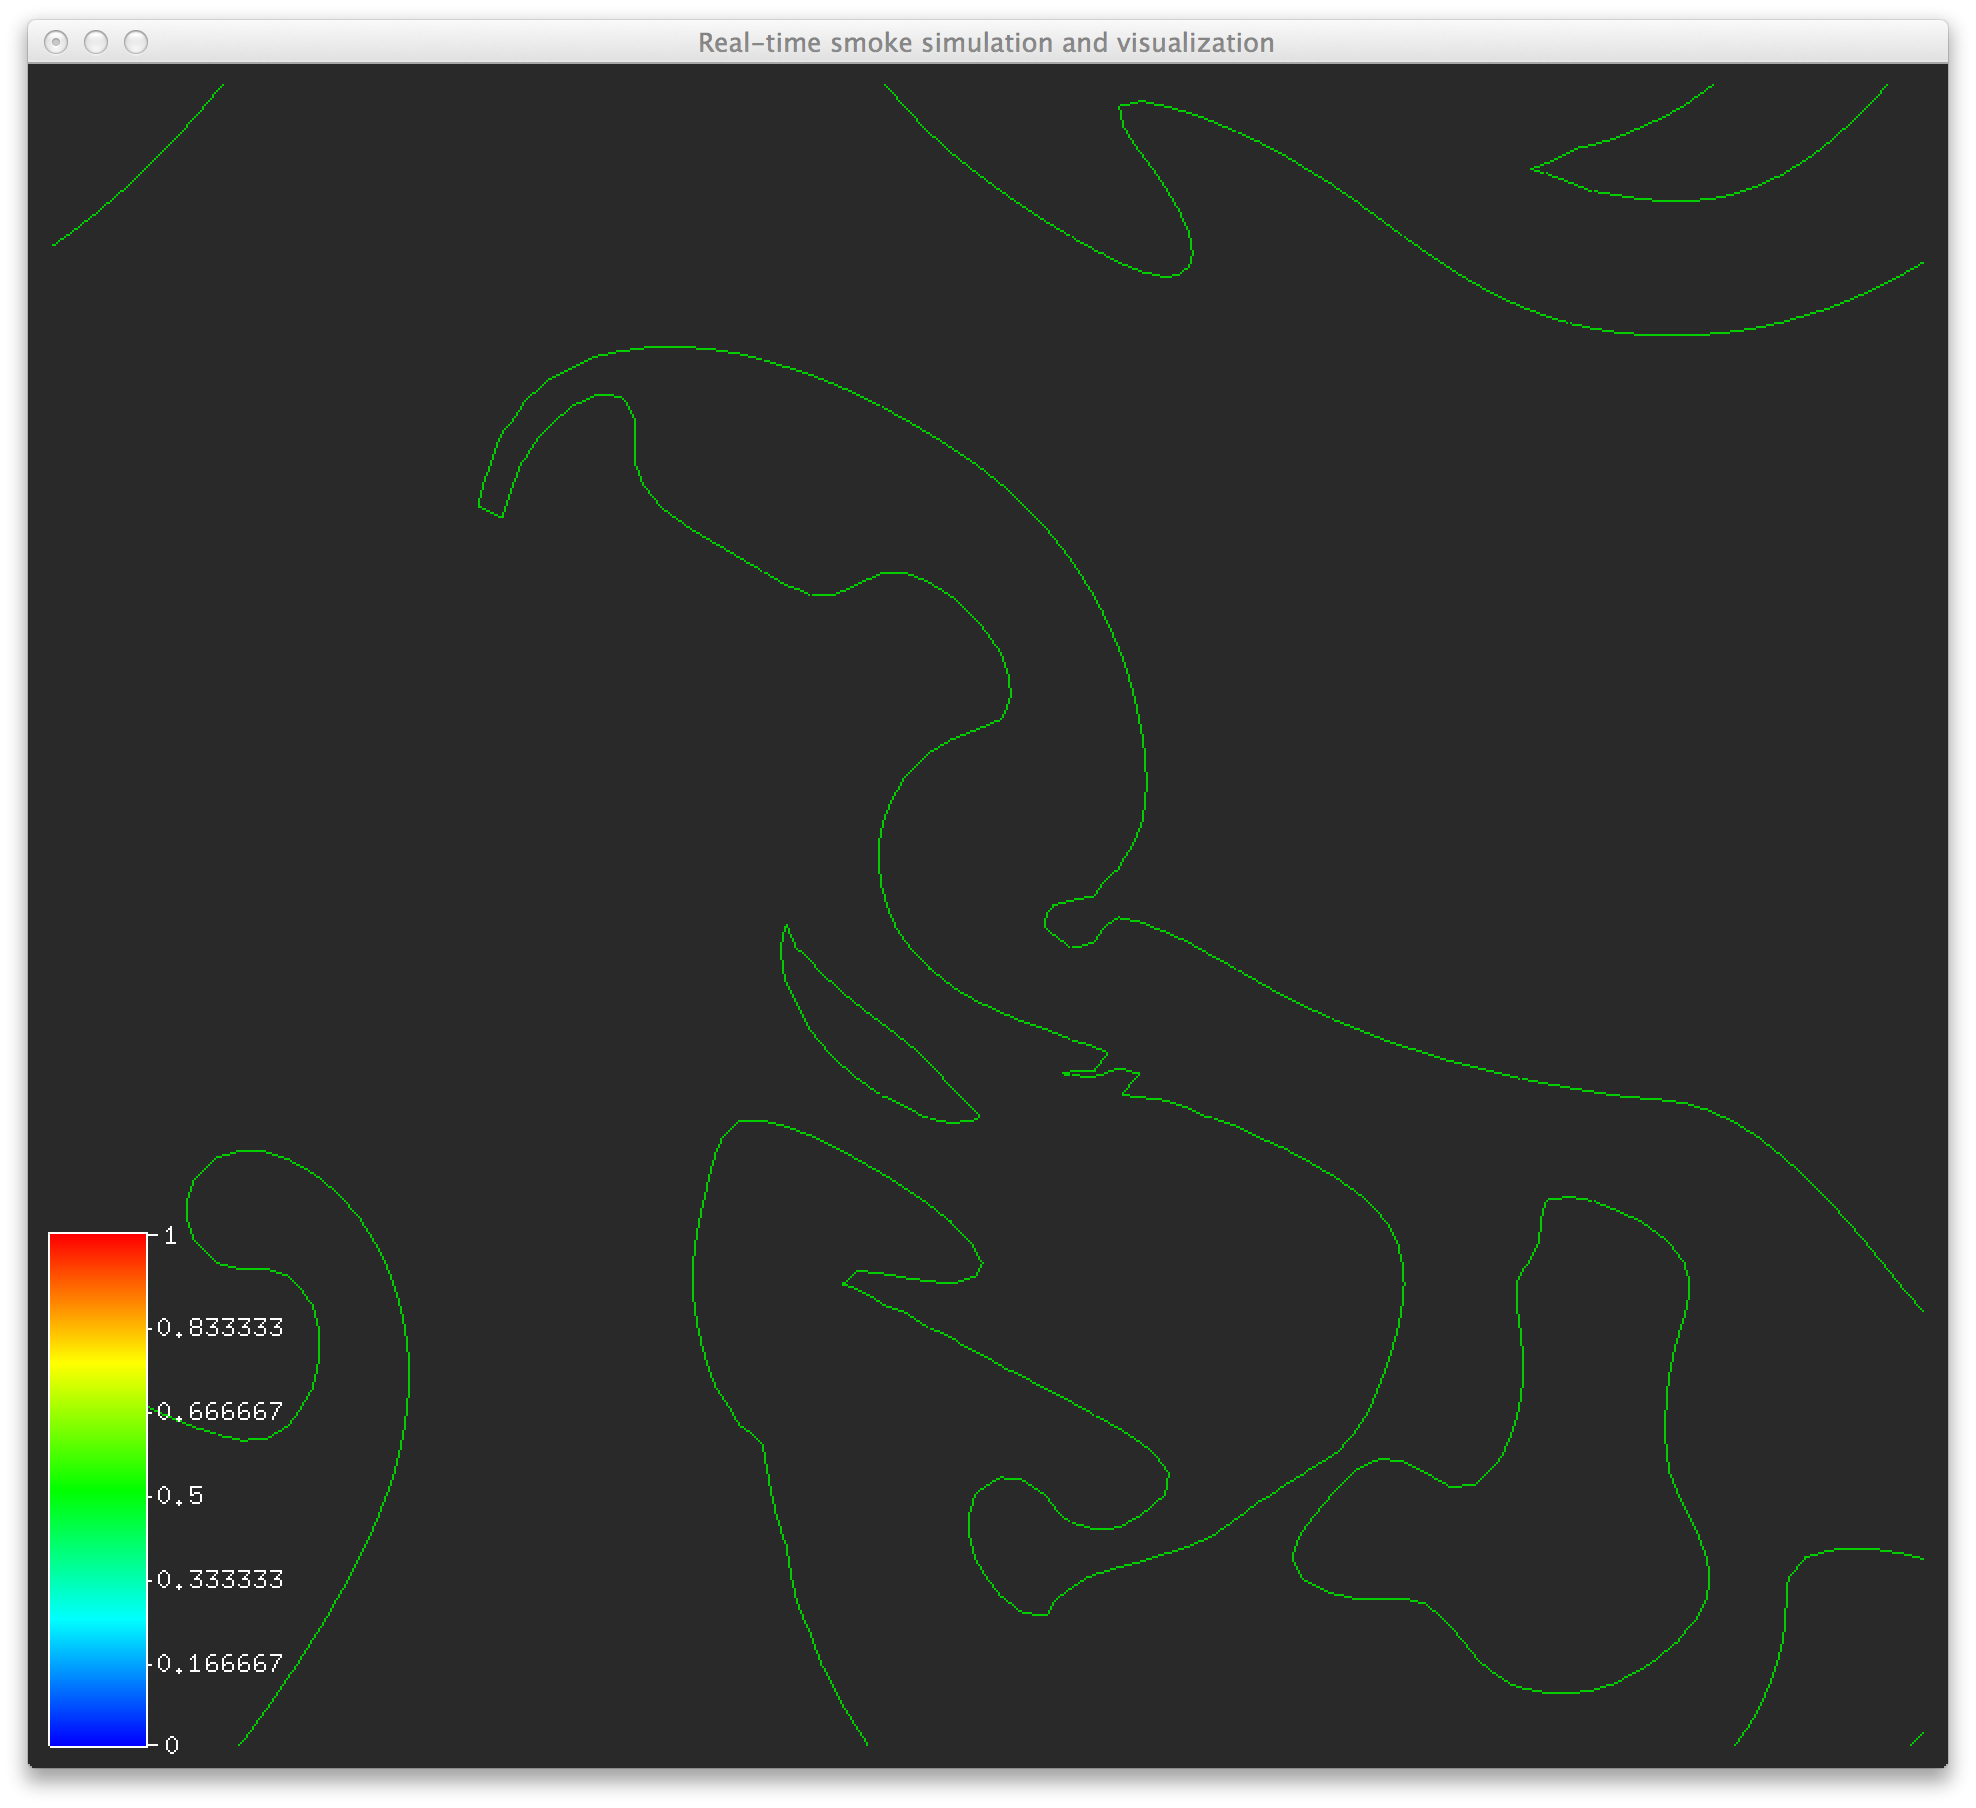
\includegraphics[height=2.7in]{figures/isolines/isoline.png}
\end{minipage}
\begin{minipage}[t]{0.48\textwidth}
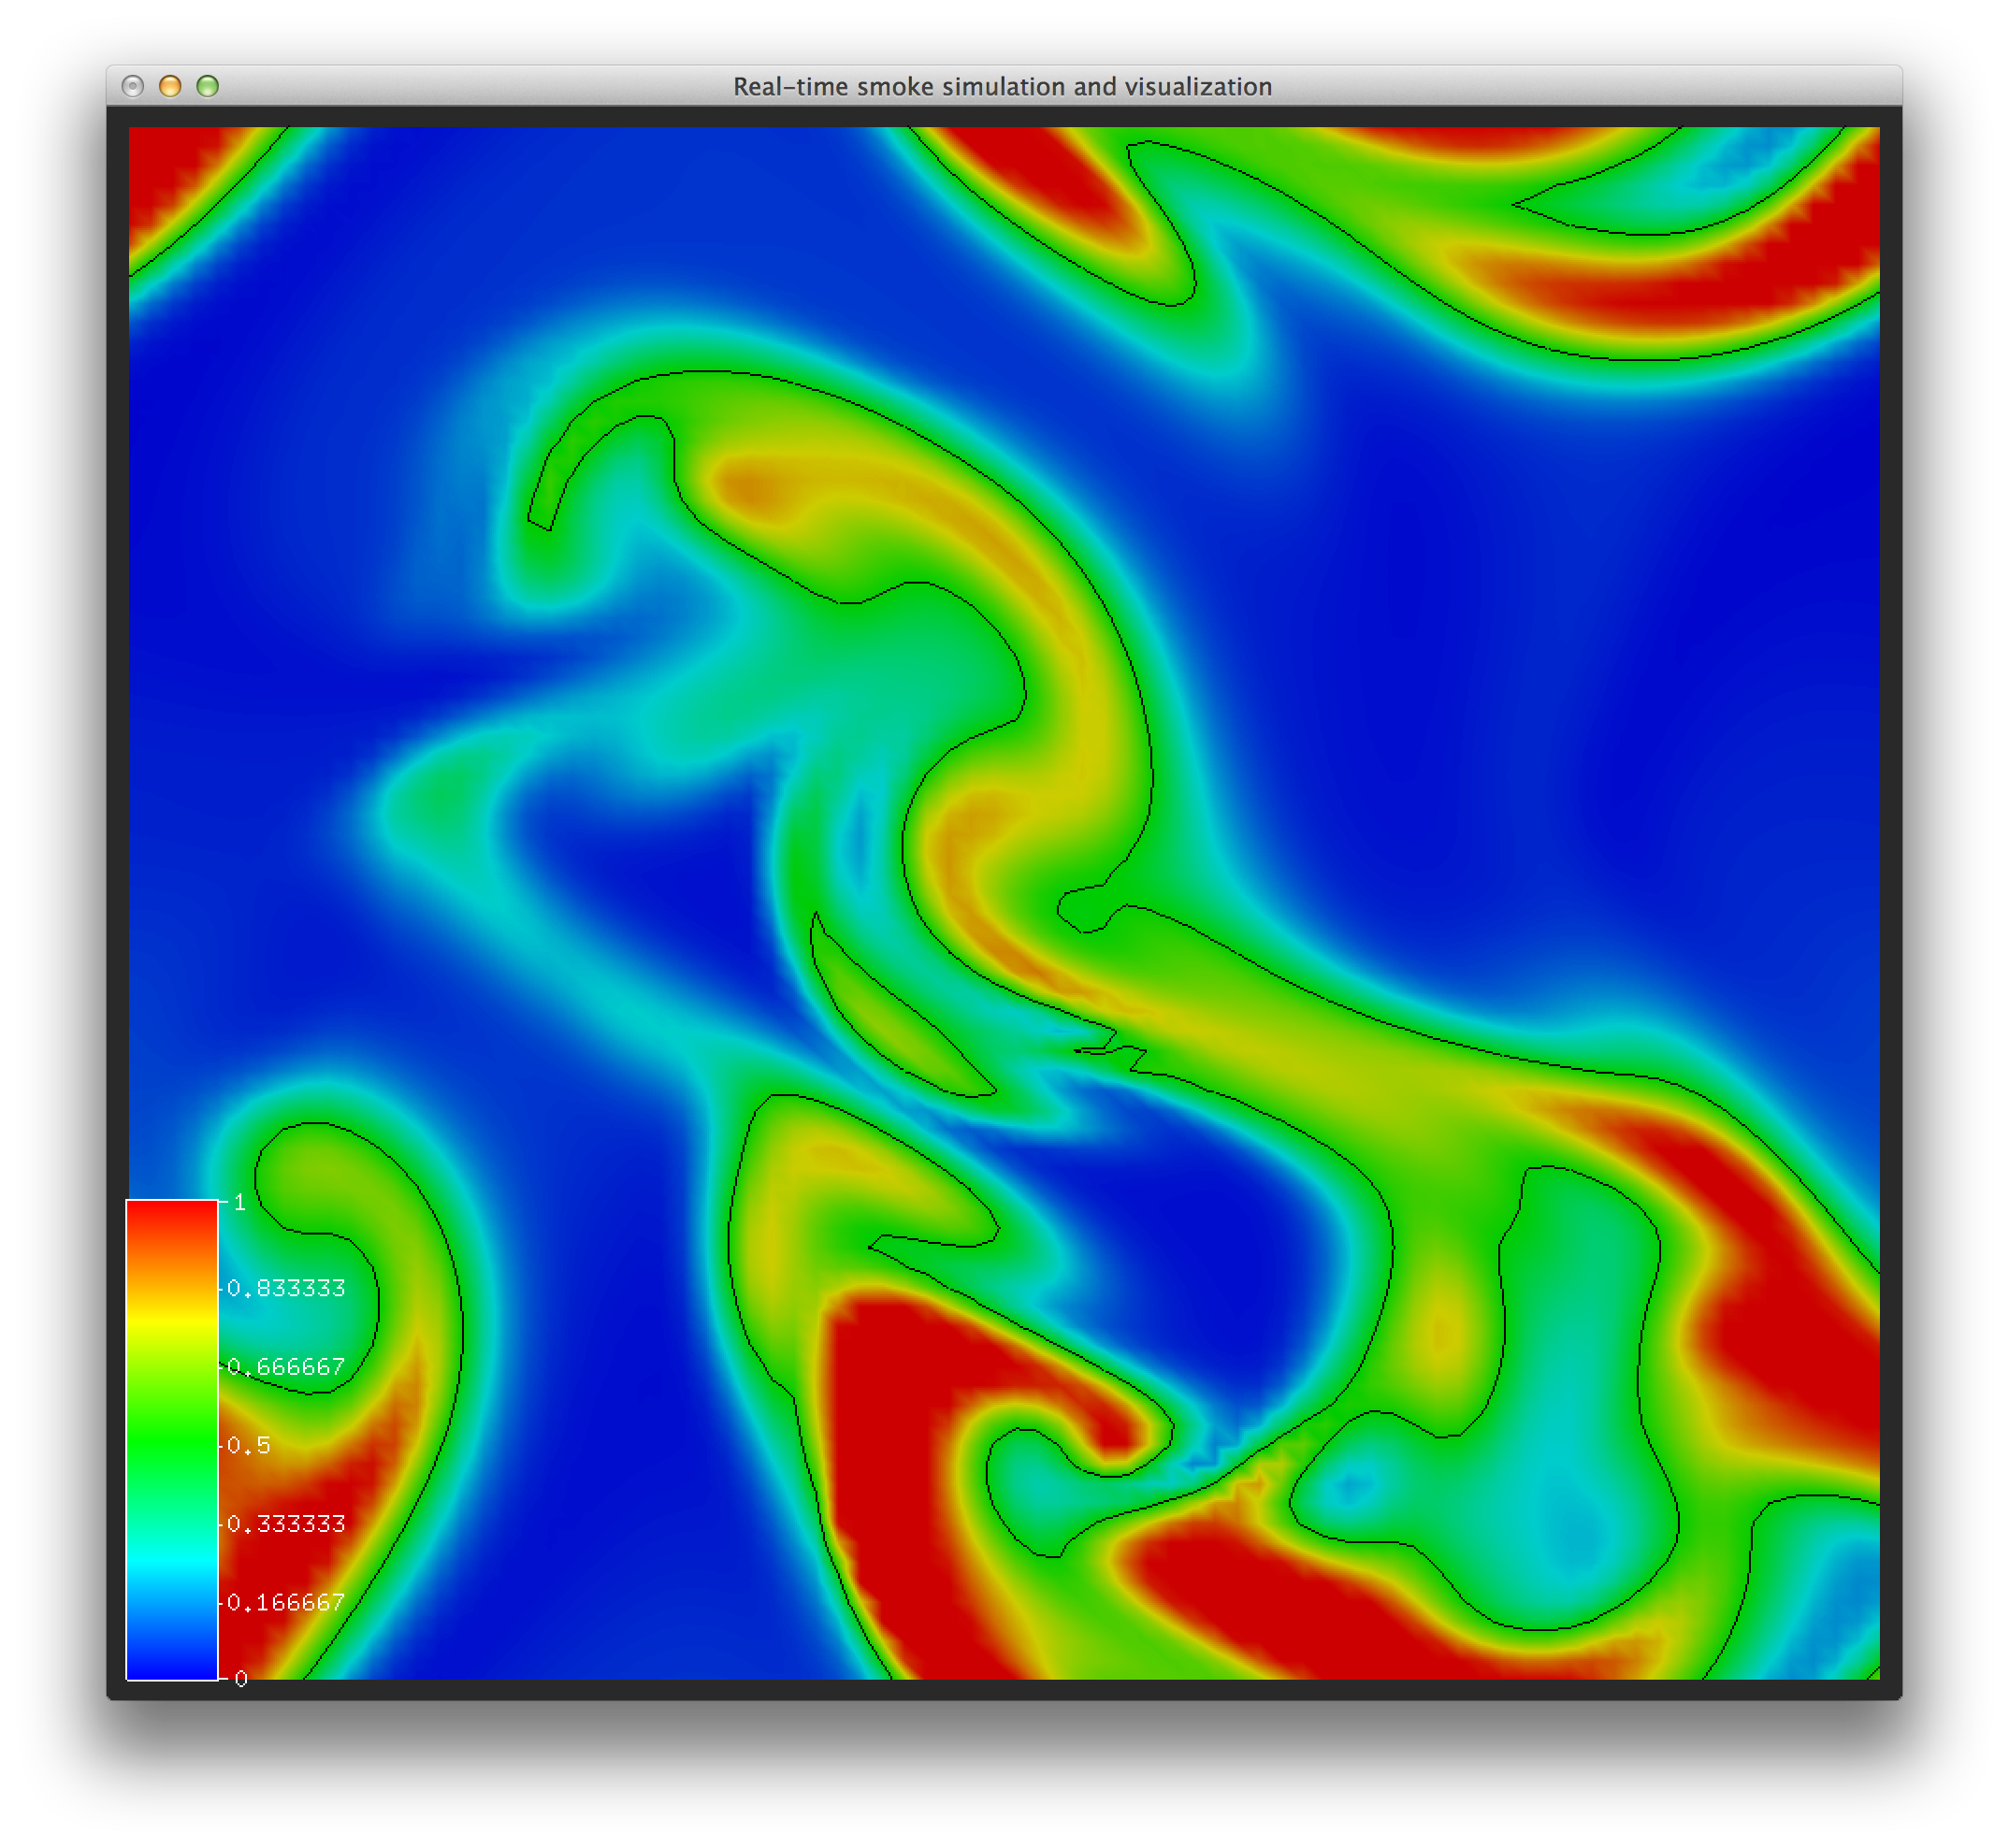
\includegraphics[height=2.7in]{figures/isolines/isolineSmoke.png}
\end{minipage}
\caption{Isolines visualisation of density value 0.5. (a) Without smoke visualisation and colorised isolines. (b) With smoke visualisation and not colorised isolines.}
\label{fig:isolineOneValue}
\end{center}
\end{figure}

The next kind of isoline visualisation lets the user select a range of density scalar values, \emph{Density rh01} and \emph{Density rho2} respectively, and the number of isolines to render equally distributed in this range. The number can be set by the control \emph{N Isolines}.